\documentclass[12pt]{article}

\usepackage{ee143report}
\usepackage{tgtermes} 
\usepackage{verbatim}
\usepackage{graphicx, float}
\usepackage{enumerate}
\usepackage{amsmath}
\usepackage[margin=1in]{geometry}
\usepackage{hyperref}

\author{Astrid Yu}
\title{PCB Design of Continuity Tester}
\expNum{4}
\titlegraphic{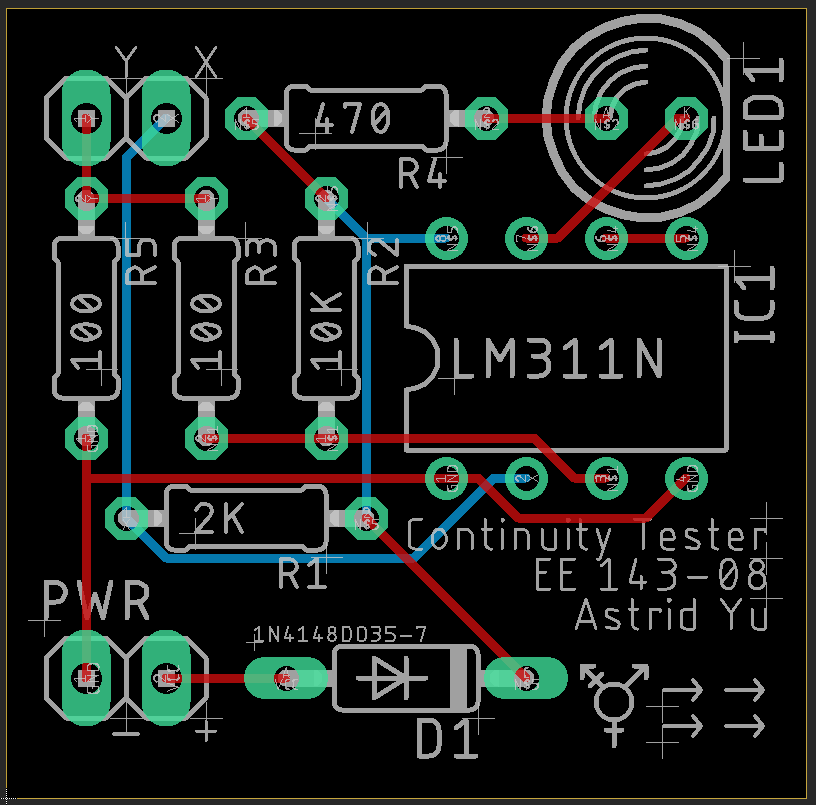
\includegraphics[width=0.6\linewidth]{pcb-top.png}}

\begin{document}
\maketitle

\section{Introduction}

The purpose of this experiment is to learn how to use computer-aided design to 
create a schematic and PCB for a continuity tester. This will primarily be done 
through Autodesk EAGLE, and the PCB will be ordered from OSHPark.

\section{Analysis}

\begin{enumerate}[a)]
    \item A schematic was created in EAGLE (Figure \ref{fig:schcr}) according to the provided schematic 
        (Figure \ref{fig:schprov}). 

        \begin{figure}[H]
            \centering
            \includegraphics[width=0.5\linewidth]{ctestsch.png}
            \caption{The provided schematic.}
            \label{fig:schprov}
        \end{figure}

        \begin{figure}[H]
            \centering
            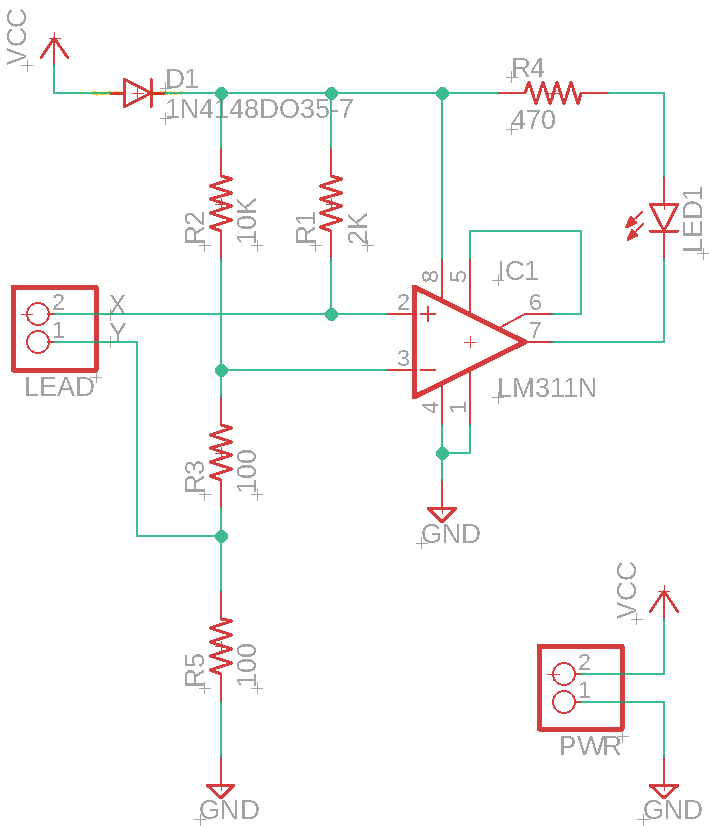
\includegraphics[width=0.4\linewidth]{sch.png}
            \caption{The created schematic.}
            \label{fig:schcr}
        \end{figure}
    \item A PCB layout was generated from the schematic (Figure \ref{fig:pcb}).  
        \begin{figure}[H]
            \centering
            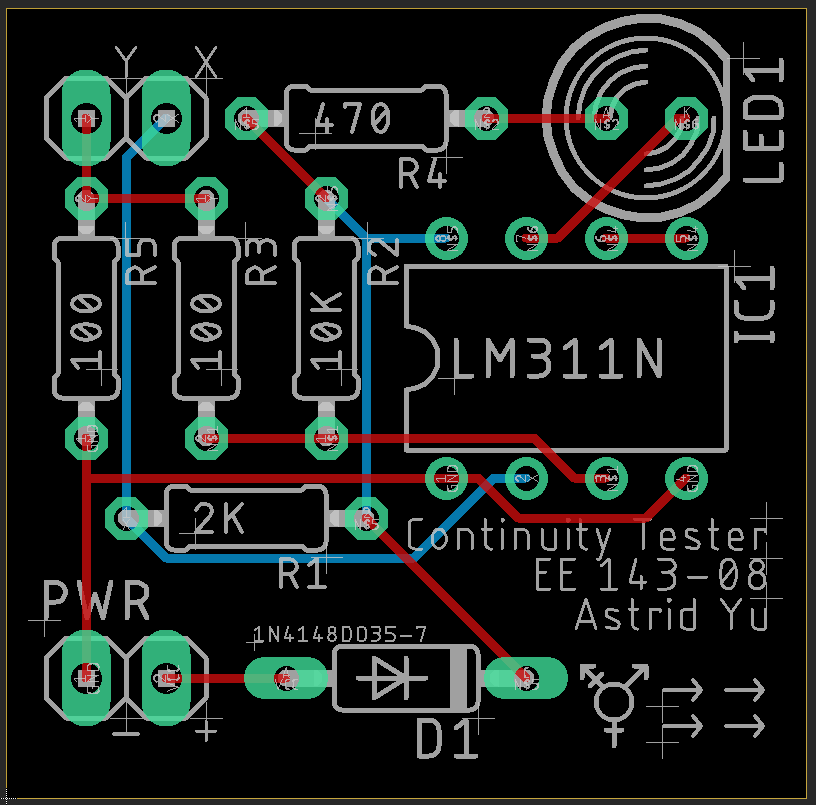
\includegraphics[width=0.4\linewidth]{pcb-top.png}
            \includegraphics[width=0.4\linewidth]{pcb-bottom.png}
            \caption{The PCB layout, top and bottom, with aesthetic modifications made to the silkscreen.}
            \label{fig:pcb}
        \end{figure}
        The PCB was verified to be correct. Optimally, this step would have been completed using 
        by printing the schematics and PCB on a physical sheet of paper, then highlighting the nodes. However, due to CoVID-19-related 
        issues obstructing accessibility to printers, this was done in Glimpse Image Editor (results in Figure \ref{fig:highlight}). 

        \begin{figure}[H]
            \centering
            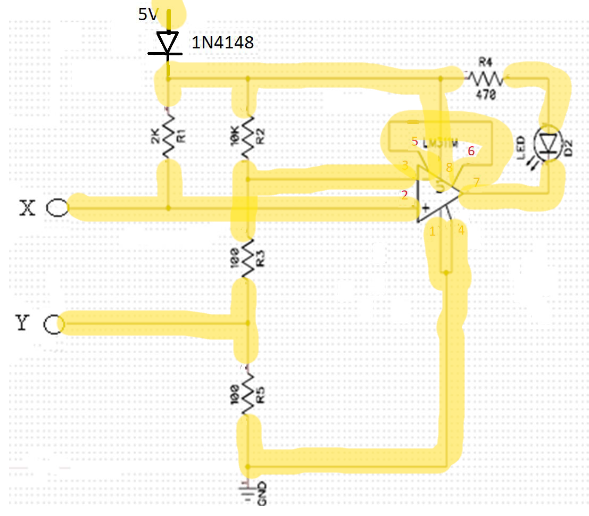
\includegraphics[width=0.3\linewidth]{ctestsch-anno.png}
            \includegraphics[width=0.3\linewidth]{sch-anno.png}
            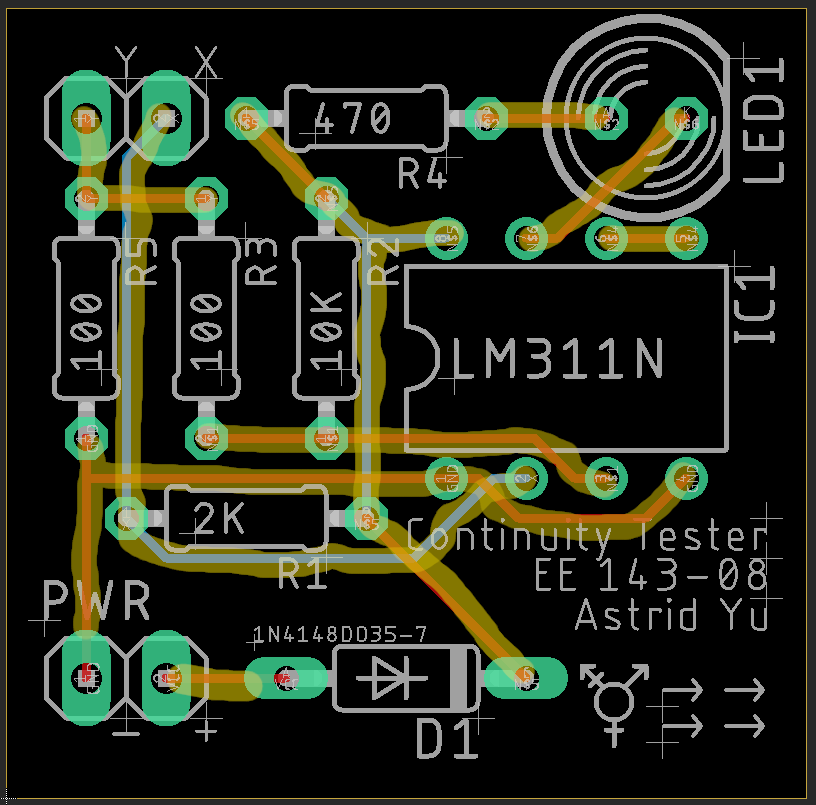
\includegraphics[width=0.3\linewidth]{pcb-anno.png}
            \caption{The results of highlighting. All nodes were found to be correct.}
            \label{fig:highlight}
        \end{figure}

        The design was uploaded to OSHPark, and a preview was generated (Figure \ref{fig:preview} and Figure \ref{fig:preview-actual})
        before the order was finalized.
        
        \begin{figure}[H]
            \centering
            \includegraphics[width=0.4\linewidth]{preview-top.png}
            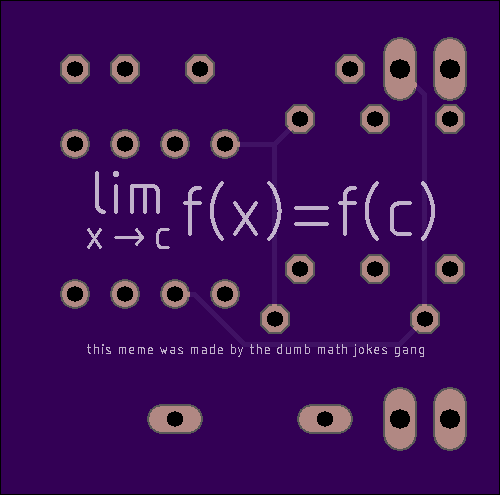
\includegraphics[width=0.4\linewidth]{preview-bottom.png}
            \caption{The previews that OSHPark generated.}
            \label{fig:preview}
        \end{figure}
        \begin{figure}[H]
            \centering
            \includegraphics[width=1in]{preview-top.png}
            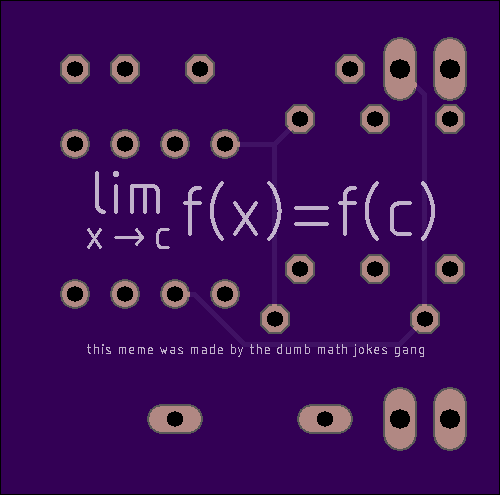
\includegraphics[width=1in]{preview-bottom.png}
            \caption{The previews that OSHPark generated, but rescaled to actual size ($1in\times 1in$).}
            \label{fig:preview-actual}
        \end{figure}
\end{enumerate}

\section{Conclusion}

A schematic was successfully entered into EAGLE, and a board was successfully generated 
from the schematic. The components were laid out and the nets were verified before 
the design was sent to production. 

Although verification and simulation can be performed on the digital schematic, it is difficult
to be completely be sure of the correctness of the design short of having it 
physically on-hand and assembling it. This highlights the importance of testing and attention
to detail prior to production.

\end{document}
